\chapter{Całki krzywoliniowe}
\label{ma2:ch:line-integrals}

Pracujemy w przestrzeni euklidesowej $\R^n$,
$n\ge1$. Rozróżniamy całkowanie względem długości
drogi, całkowanie względem miary Hausdorffa jej
obrazu oraz całkowanie zorientowane.
Podstawą jest teoria krzywych prostowalnych
z rozdziału \ref{ma2:ch:rectifiable-curves}.
Nie zakładamy, że krzywa jest różnowartościowa.

\section{Całka krzywoliniowa pierwszego rodzaju}

\begin{definicja}
\label{ma2:def:line-first}
Niech $\gamma:[a,b]\to\R^n$, $a<b$, będzie
ciągła i prostowalna, $\ell=L(\gamma)$, a
$\widehat\gamma:[0,\ell]\to\R^n$ jej parametryzacją
długością łuku z \ref{ma2:thm:curve-arclength}.
Oznaczmy $E=\gamma([a,b])$.
Dla nieujemnej funkcji borelowskiej $f$ na $E$
określamy całkę krzywoliniową pierwszego rodzaju
\[
 I_\gamma(f)=\int_{[0,\ell]} f(\widehat\gamma(s))\,
 \mathrm d\lambda_1(s).
\]
Dla rzeczywistej funkcji borelowskiej $f$ stosujemy
tę samą definicję, jeśli $I_\gamma(|f|)<\infty$.
Klasyczne oznaczenie $\int_\gamma f\,\mathrm ds$
oznacza właśnie $I_\gamma(f)$.
Dla $\ell=0$ całka wynosi zero.
\end{definicja}

Składanie funkcji borelowskiej z ciągłą
parametryzacją daje funkcję borelowską.
Dla $f=1$ całka jest równa $\ell$.
Dla ograniczonej funkcji $f$ mamy
$|I_\gamma(f)|\le \ell\sup_E|f|$,
na mocy oszacowania całki Lebesgue'a.
Liniowość na funkcjach całkowalnych,
monotoniczność i twierdzenia graniczne
wynikają bezpośrednio z odpowiednich własności
całki Lebesgue'a.

\begin{twierdzenie}[Całka względem miary Hausdorffa z krotnością]
\label{ma2:thm:line-weighted-area}
Dla krzywej ciągłej prostowalnej i funkcji
$f$ z definicji \ref{ma2:def:line-first} zachodzi
\[
 I_\gamma(f)=\int_E f(y)N_\gamma(y)\,
 \mathrm d\mathcal H^1(y),
\]
gdzie $N_\gamma(y)=\#\gamma^{-1}(\{y\})$,
z wartością $+\infty$ dla nieskończonego włókna.
Przyjmujemy $0\cdot(+\infty)=0$.
W szczególności gdy $N_\gamma=1$
$\mathcal H^1$-prawie wszędzie na $E$,
\[
 I_\gamma(f)=\int_E f\,\mathrm d\mathcal H^1.
\]
\end{twierdzenie}
\begin{proof}
Dla $\ell=0$ obraz jest punktem miary zero,
więc obie całki są zerowe.
Niech $\ell>0$ i najpierw $f\ge0$.
Parametryzację $\widehat\gamma$ przedłużamy
stałymi wartościami poza $[0,\ell]$;
przedłużenie jest $1$-Lipschitzowskie.
Z \ref{ma2:thm:curve-arclength} mamy
$\|\widehat\gamma'(s)\|_2=1$ prawie wszędzie.
Stosujemy ważony wzór na pole z krotnością
(\atlasref{ME-28::thm:lipschitz-area-coarea-28}{ME 28})
dla zbioru $[0,\ell]$ i wagi
$f\circ\widehat\gamma$. Jednowymiarowy
jakobian jest równy normie pochodnej.
Otrzymujemy
\[
 I_\gamma(f)=\int_E f(y)N_{\widehat\gamma}(y)\,
 \mathrm d\mathcal H^1(y).
\]
W dowodzie \ref{ma2:thm:curve-length-multiplicity}
wykazano, że $N_{\widehat\gamma}=N_\gamma$
poza zbiorem przeliczalnym, a więc zerowym
względem $\mathcal H^1$.
Dla funkcji rzeczywistych stosujemy wynik
do części dodatniej i ujemnej; skończoność
całki z $|f|$ pozwala odjąć obie równości.
\end{proof}

Całka względem $\mathcal H^1$ na obrazie
nie uwzględnia wielokrotnych przejść przez
ten sam łuk. Całka pierwszego rodzaju
uwzględnia je przez funkcję krotności.
Na krzywej zamkniętej jednokrotne powtórzenie
punktu początkowego na końcu nie zmienia całki.

\begin{lemat}[Miara obrazowa parametru długości]
\label{ma2:lem:line-arclength-push}
Niech $\gamma$ będzie absolutnie ciągła,
a $s(t)=L_{[a,t]}(\gamma)$ i $\ell=s(b)$.
Dla każdej nieujemnej funkcji borelowskiej $h$
na $[0,\ell]$ zachodzi
\[
 \int_{[0,\ell]}h(u)\,\mathrm d\lambda_1(u)
 =\int_{[a,b]}h(s(t))s'(t)\,\mathrm d\lambda_1(t).
\]
Ta sama równość zachodzi dla całkowalnej
rzeczywistej funkcji borelowskiej $h$.
\end{lemat}
\begin{proof}
Z \ref{ma2:thm:curve-ac-length} wynika, że
$s$ jest absolutnie ciągła i niemalejąca,
$s(a)=0$, $s(b)=\ell$, a
$s'=\|\gamma'\|_2$ prawie wszędzie.
Na zbiorze wyjątkowym przyjmujemy $s'=0$.
Dla $0\le q\le\ell$ zbiór
$\{t:s(t)\le q\}$ jest przedziałem $[a,t_q]$,
gdzie $t_q$ jest największym punktem włókna
$s^{-1}(\{q\})$. Z absolutnej ciągłości
\[
 \int_{[a,t_q]}s'(t)\,\mathrm d\lambda_1(t)
 =s(t_q)-s(a)=q.
\]
Zatem miara obrazowa miary
$s'\lambda_1|_{[a,b]}$ przez $s$
i miara Lebesgue'a na $[0,\ell]$ mają te same
wartości na przedziałach $[0,q]$.
Są to skończone miary, więc zgodność na tej
rodzinie generującej zbiory borelowskie
daje ich równość. Wzór na całkę względem
miary obrazowej
(\atlasref{ME-13::thm:pushforward-integral-13}{ME 13})
daje tezę. Obejmuje ona też $\ell=0$.
\end{proof}

\begin{wniosek}[Wzór w dowolnym parametrze absolutnie ciągłym]
\label{ma2:cor:line-first-speed}
Jeżeli $\gamma$ jest absolutnie ciągła, to
\[
 I_\gamma(f)=\int_{[a,b]} f(\gamma(t))
 \|\gamma'(t)\|_2\,\mathrm d\lambda_1(t).
\]
\end{wniosek}
\begin{proof}
Stosujemy \ref{ma2:lem:line-arclength-push}
do $h=f\circ\widehat\gamma$ i korzystamy
z faktoryzacji $\gamma=\widehat\gamma\circ s$.
\end{proof}
W szczególności dla krzywej ciągłej kawałkami
klasy $C^1$ na skończonym podziale można
obliczać całkę przez całki na poszczególnych
częściach. Taka krzywa jest absolutnie ciągła:
na każdej części jej pochodna jest ograniczona,
a nierówność wartości średniej i sumowanie
oszacowań przez punkty podziału dają globalną
własność Lipschitza.

Wzoru z pochodną nie wolno stosować do każdej
krzywej ciągłej prostowalnej. Krzywa z funkcją
Cantora z \ref{ma2:ex:curve-cantor} ma długość
$1$, mimo że jej pochodna jest zerowa
prawie wszędzie. Dla $f=1$ wzór
\ref{ma2:cor:line-first-speed} bez hipotezy
absolutnej ciągłości dawałby błędny wynik.

\section{Całka krzywoliniowa drugiego rodzaju}

\begin{definicja}
\label{ma2:def:line-second}
Niech $\gamma:[a,b]\to\R^n$ będzie ciągła
i prostowalna, $E=\gamma([a,b])$, a
$F:E\to\R^n$ pole ciągłe.
Całkę krzywoliniową drugiego rodzaju określamy
przez
\[
 W_\gamma(F)=\int_{[0,\ell]}
 \langle F(\widehat\gamma(s)),\widehat\gamma'(s)\rangle
 \,\mathrm d\lambda_1(s).
\]
Pochodną przyjmujemy równą zero na zbiorze
wyjątkowym miary zero, a dla $\ell=0$
całą całkę przyjmujemy równą zero.
Klasyczne oznaczenie to
$\int_\gamma\sum_{j=1}^n F_j\,\mathrm dx_j$.
\end{definicja}

Funkcja podcałkowa jest mierzalna
i ograniczona prawie wszędzie przez
$\sup_E\|F\|_2$, ponieważ $E$ jest zwarty,
a parametryzacja długością łuku ma
prędkość jednostkową prawie wszędzie.
W szczególności
\[
 |W_\gamma(F)|\le I_\gamma(\|F\|_2)
 \le L(\gamma)\sup_E\|F\|_2.
\]
Pierwsza nierówność wynika z nierówności
Cauchy'ego--Schwarza i nierówności trójkąta
dla całki, druga z definicji całki
pierwszego rodzaju.

\begin{twierdzenie}[Całka drugiego rodzaju w parametrze absolutnie ciągłym]
\label{ma2:thm:line-second-speed}
Jeżeli $\gamma$ jest absolutnie ciągła,
to
\[
 W_\gamma(F)=\int_{[a,b]}
 \langle F(\gamma(t)),\gamma'(t)\rangle
 \,\mathrm d\lambda_1(t).
\]
Równoważnie
\[
 W_\gamma(F)=\sum_{j=1}^n
 \int_{[a,b]}F_j(\gamma(t))\gamma_j'(t)
 \,\mathrm d\lambda_1(t).
\]
\end{twierdzenie}
\begin{proof}
Niech $s$ będzie funkcją długości.
Na zbiorze punktów różniczkowalności $s$
z $s'(t)=0$ własność Lipschitza
$\widehat\gamma$ daje
\[
 \frac{\|\gamma(t+h)-\gamma(t)\|_2}{|h|}
 \le \frac{|s(t+h)-s(t)|}{|h|}\longrightarrow0.
\]
W tych punktach $\gamma'(t)=0$.
Niech $B\subseteq[0,\ell]$ będzie borelowskim
zbiorem miary zero zawierającym końce przedziału
i wszystkie punkty, w których
$\widehat\gamma'$ nie istnieje.
Z \ref{ma2:lem:line-arclength-push} dla $h=\chi_B$
wynika
\[
 \int_{s^{-1}(B)}s'(t)\,\mathrm d\lambda_1(t)=0.
\]
Ponieważ $s'\ge0$ prawie wszędzie, zbiór
punktów z $s(t)\in B$ i $s'(t)>0$
ma miarę zero. W pozostałych punktach,
w których $s'(t)>0$, stosujemy regułę
łańcuchową. Łącznie dostajemy
$\gamma'(t)=\widehat\gamma'(s(t))s'(t)$
prawie wszędzie, przyjmując pochodną
$\widehat\gamma$ równą zero na $B$.
Można wybrać borelowskiego przedstawiciela
tej pochodnej, na przykład przez granice
ilorazów różnicowych z krokiem dążącym do zera
i przypisanie zera na zbiorze wyjątkowym.
Stosujemy teraz \ref{ma2:lem:line-arclength-push}
do ograniczonej funkcji
$h(u)=\langle F(\widehat\gamma(u)),
\widehat\gamma'(u)\rangle$.
Druga równość wynika z definicji iloczynu
skalarnego i liniowości całki.
\end{proof}

\section{Reparametryzacja, orientacja i składanie dróg}

\begin{twierdzenie}
\label{ma2:thm:line-orientation}
Niech $\varphi:[c,d]\to[a,b]$, $c<d$,
będzie ciągłą monotoniczną surjekcją.
Dla $\eta=\gamma\circ\varphi$ zachodzi
$I_\eta(f)=I_\gamma(f)$.
Dla pola ciągłego zachodzi
\[
 W_\eta(F)=
 \begin{cases}
 W_\gamma(F),&\varphi\text{ niemalejąca},\\
 -W_\gamma(F),&\varphi\text{ nierosnąca}.
 \end{cases}
\]
\end{twierdzenie}
\begin{proof}
Niech $s_\gamma,s_\eta$ oznaczają funkcje
długości odpowiednich krzywych.
Z niezmienniczości długości
(\ref{ma2:thm:curve-reparam}) na podprzedziałach
otrzymujemy dla niemalejącej $\varphi$
$s_\eta(t)=s_\gamma(\varphi(t))$.
Dla nierosnącej $\varphi$ addytywność długości
daje $s_\eta(t)=\ell-s_\gamma(\varphi(t))$.
Jeżeli ograniczenie $\varphi$ jest stałe,
odpowiednie długości są zerowe i wzory
nadal zachodzą.
Z jednoznaczności faktoryzacji przez długość
łuku wynika odpowiednio
$\widehat\eta(u)=\widehat\gamma(u)$ albo
$\widehat\eta(u)=\widehat\gamma(\ell-u)$.
Pierwszy przypadek jest natychmiastowy.
W drugim podstawienie $v=\ell-u$ zachowuje
całkę pierwszego rodzaju, natomiast
$\widehat\eta'(u)=-\widehat\gamma'(\ell-u)$
prawie wszędzie zmienia znak całki
drugiego rodzaju.
Dla $\ell=0$ wszystkie całki są zerowe.
\end{proof}

\begin{stwierdzenie}[Addytywność]
\label{ma2:prop:line-additivity}
Niech $a<t<b$ oraz
$\gamma_1=\gamma|_{[a,t]}$,
$\gamma_2=\gamma|_{[t,b]}$.
Wtedy
\[
 I_\gamma(f)=I_{\gamma_1}(f)+I_{\gamma_2}(f),
 \qquad
 W_\gamma(F)=W_{\gamma_1}(F)+W_{\gamma_2}(F).
\]
Pierwsza równość obowiązuje dla nieujemnych
funkcji borelowskich lub funkcji całkowalnych
względem długości.
\end{stwierdzenie}
\begin{proof}
Niech $\ell_1=L(\gamma_1)$.
Z addytywności długości i jednoznaczności
parametryzacji długością łuku
wynika, że $\widehat\gamma_1$ jest
ograniczeniem $\widehat\gamma$ do $[0,\ell_1]$,
a $\widehat\gamma_2(u)=\widehat\gamma(\ell_1+u)$
dla $0\le u\le\ell-\ell_1$.
Dzielimy całki na te dwa przedziały.
Ich wspólny koniec ma miarę zero;
jeśli jedna część ma długość zero,
jej wkład także jest zerowy.
\end{proof}

Dla dwóch dróg $\gamma_1:[a,b]\to\R^n$
oraz $\gamma_2:[c,d]\to\R^n$ z
$\gamma_1(b)=\gamma_2(c)$ definiujemy
ich złożenie przez przejście najpierw
wzdłuż $\gamma_1$, następnie $\gamma_2$,
po afinicznych rosnących reparametryzacjach
na $[0,1]$ i $[1,2]$.
Z poprzednich wyników całka po złożonej
drodze jest sumą całek po jej częściach.

\begin{przyklad}[Przejście i powrót]
\label{ma2:ex:line-backtrack}
Niech $\gamma$ będzie drogą prostowalną,
a $\gamma^{-}$ tą samą drogą z odwróconym
parametrem. Dla złożenia $\eta$ drogi $\gamma$
i jej odwrotności, przy $f\ge0$ lub
$I_\gamma(|f|)<\infty$, mamy
\[
 I_\eta(f)=2I_\gamma(f),\qquad W_\eta(F)=0.
\]
Wynika to z \ref{ma2:thm:line-orientation}
oraz \ref{ma2:prop:line-additivity}.
Długość drogi podwaja się, mimo że całka
zorientowana znika dla każdego pola ciągłego.
\end{przyklad}

\section{Formy stopnia pierwszego i funkcje pierwotne}

Na zbiorze otwartym $U\subseteq\R^n$
ciągłe pole $F:U\to\R^n$ wyznacza ciągłe
pole kowektorów
\[
 \omega_x(v)=\langle F(x),v\rangle,\qquad
 \omega=\sum_{j=1}^nF_j\,\mathrm dx_j .
\]
Dla gładkich współczynników jest to forma
różniczkowa stopnia pierwszego w sensie
\atlasref{DG-10::def:forma-rozniczkowa}{DG 10}.
Dla krzywej klasy $C^1$ cofnięcie formy
jest dane wzorem
\[
 \gamma^*\omega=
 \left(\sum_{j=1}^n F_j(\gamma(t))\gamma_j'(t)\right)
 \mathrm dt,
\]
gdzie $\mathrm dt$ oznacza kowektor na
prostej parametru, nie miarę.
Wzór wynika z definicji cofnięcia
\atlasref{DG-10::prop:formy-wedge-pullback}{DG 10}.
Całkowanie współczynnika tego cofnięcia
względem $\lambda_1$ daje
$W_\gamma(F)$ na mocy
\ref{ma2:thm:line-second-speed}.
W szczególności nie wprowadza się modułu
pochodnej w całce zorientowanej.

\begin{twierdzenie}[Twierdzenie o funkcji pierwotnej]
\label{ma2:thm:line-fundamental}
Niech $U\subseteq\R^n$ będzie otwarty,
$P:U\to\R$ klasy $C^1$, a $\gamma$
ciągłą krzywą prostowalną w $U$.
Wówczas
\[
 W_\gamma(\nabla P)=P(\gamma(b))-P(\gamma(a)).
\]
\end{twierdzenie}
\begin{proof}
Dla $\ell=0$ obie strony są zerowe.
Dla $\ell>0$ funkcja $P\circ\widehat\gamma$
jest absolutnie ciągła. Istotnie, zwarty
obraz krzywej można pokryć skończenie wieloma
otwartymi kulami, na których $P$ jest
Lipschitzowska dzięki lokalnemu ograniczeniu
gradientu. Jednostajna ciągłość
$\widehat\gamma$ i lemat o liczbie Lebesgue'a
dla pokrycia przedziału przeciwobrazami tych kul
dają własność Lipschitza z jednolitą stałą
dla dostatecznie bliskich parametrów.
Dzieląc dowolny przedział parametrów na
dostatecznie krótkie części otrzymujemy
globalną własność Lipschitza.
Reguła łańcuchowa w punktach
różniczkowalności $\widehat\gamma$
daje prawie wszędzie
\[
 (P\circ\widehat\gamma)'(s)=
 \langle\nabla P(\widehat\gamma(s)),
 \widehat\gamma'(s)\rangle .
\]
Twierdzenie o funkcji pierwotnej dla
funkcji absolutnie ciągłych
(\atlasref{AM1-37::ma1:kh:thm:ac-lebesgue-primitive}{AM I, rozdział 37})
daje wynik.
\end{proof}

\begin{twierdzenie}[Niezależność całki od drogi]
\label{ma2:thm:line-path-independence}
Niech $U\subseteq\R^n$ będzie niepustym
otwartym zbiorem spójnym, a $F:U\to\R^n$
polem ciągłym. Następujące warunki są równoważne:
\begin{enumerate}
\item Istnieje $P\in C^1(U,\R)$ takie, że
$F=\nabla P$.
\item Całki $W_\gamma(F)$ po dowolnych dwóch
ciągłych krzywych prostowalnych w $U$
o tych samych uporządkowanych końcach są równe.
\item Dla każdej zamkniętej ciągłej krzywej
prostowalnej w $U$ zachodzi $W_\gamma(F)=0$.
\end{enumerate}
\end{twierdzenie}
\begin{proof}
Implikacja (1)$\Rightarrow$(2) wynika z
\ref{ma2:thm:line-fundamental}, a (2)$\Rightarrow$(3)
z porównania drogi zamkniętej z drogą stałą.
Z (3) wynika (2) przez złożenie pierwszej
drogi z odwróceniem drugiej.

Ustalmy $x_0\in U$. Każdy punkt $U$ można
połączyć z $x_0$ łamaną leżącą w $U$:
zbiór osiągalnych punktów jest niepusty
i względnie otwarty, ponieważ przy każdym
punkcie istnieje kula zawarta w $U$,
a odcinki w tej kuli pozostają w $U$.
Tak samo jego dopełnienie jest względnie
otwarte, gdyż gdyby w kuli wokół punktu
nieosiągalnego istniał punkt osiągalny,
odcinek łączyłby je. Spójność daje tezę.
Z (2) możemy określić
$P(x)=W_{\gamma_x}(F)$, gdzie $\gamma_x$
jest dowolną taką drogą od $x_0$ do $x$.
Dla małego $h\in\R^n$, takiego że
odcinek od $x$ do $x+h$ leży w $U$,
z addytywności i wzoru
\ref{ma2:thm:line-second-speed} mamy
\[
 P(x+h)-P(x)=\int_0^1
 \langle F(x+th),h\rangle\,\mathrm d\lambda_1(t).
\]
Odejmując $\langle F(x),h\rangle$,
otrzymujemy resztę o module nie większym niż
\[
 \|h\|_2\sup_{0\le t\le1}\|F(x+th)-F(x)\|_2
 =o(\|h\|_2)
\]
dzięki ciągłości $F$. Zatem $DP(x)$ jest
kowektorem $h\mapsto\langle F(x),h\rangle$,
a ciągłość $F$ daje $P\in C^1(U,\R)$.
\end{proof}

Pole spełniające te warunki nazywamy
polem zachowawczym. Funkcja pierwotna
jest wyznaczona z dokładnością do stałej
na zbiorze spójnym: różnica dwóch funkcji
pierwotnych ma gradient zerowy, a
\ref{ma2:thm:line-fundamental} na łamanych
daje stałość różnicy.

\begin{twierdzenie}[Kryterium na zbiorze gwiaździstym]
\label{ma2:thm:line-star-shaped}
Niech $U\subseteq\R^n$ będzie otwarty
i gwiaździsty względem $p\in U$,
to znaczy $[p,x]\subset U$ dla każdego $x\in U$.
Dla $F\in C^1(U,\R^n)$ istnieje funkcja
pierwotna wtedy i tylko wtedy, gdy
\[
 \partial_i F_j=\partial_j F_i
 \qquad(1\le i,j\le n).
\]
\end{twierdzenie}
\begin{proof}
Jeżeli $F=\nabla P$, to $P$ jest klasy $C^2$,
a równość wynika z twierdzenia Schwarza.
Odwrotnie określamy
\[
 P(x)=\int_0^1
 \sum_{j=1}^n F_j(p+t(x-p))(x_j-p_j)
 \,\mathrm d\lambda_1(t).
\]
Jest to całka po odcinku od $p$ do $x$.
Różniczkujemy względem $x_i$ pod całką:
dla ustalonego $x$ zwarty odcinek $[p,x]$
ma dodatnią odległość od dopełnienia $U$
(jeśli $U=\R^n$, wystarczy dowolne ograniczone
otoczenie odcinka). Dla $x'$ dostatecznie
bliskich $x$ wszystkie odpowiednie odcinki
leżą w tym samym zwartym podzbiorze $U$.
Ciągłość $F$ i jego pochodnych daje
jednolite ograniczenie funkcji podcałkowej
oraz pochodnych względem $x'$,
więc stosujemy twierdzenie o różniczkowaniu
całki zależnej od parametru z rozdziału
\ref{ma2:ch:parameter-integrals}.
Piszemy $q_t=p+t(x-p)$ i otrzymujemy
\[
 \begin{aligned}
 \partial_iP(x)
 &=\int_0^1\left(F_i(q_t)+
 t\sum_j\partial_iF_j(q_t)(x_j-p_j)\right)
 \mathrm d\lambda_1(t)\\
 &=\int_0^1\left(F_i(q_t)+
 t\sum_j\partial_jF_i(q_t)(x_j-p_j)\right)
 \mathrm d\lambda_1(t)\\
 &=\int_0^1\frac{\mathrm d}{\mathrm dt}
 \bigl(tF_i(q_t)\bigr)\,\mathrm d\lambda_1(t)
 =F_i(x).
 \end{aligned}
\]
Ostatni krok to podstawowe twierdzenie
rachunku całkowego. Stąd $P$ jest klasy $C^1$
i $\nabla P=F$.
\end{proof}

\section{Przykłady obliczeniowe}

\begin{przyklad}[Całka z funkcji skalarnej po okręgu]
\label{ma2:ex:line-circle-first}
Niech $\gamma(t)=(R\cos t,R\sin t)$,
$0\le t\le2\pi$, $R>0$.
Dla $f(x,y)=x^2$ mamy
\[
 I_\gamma(f)=R^3\int_0^{2\pi}\cos^2t\,
 \mathrm d\lambda_1(t)=\pi R^3
\]
na mocy \ref{ma2:cor:line-first-speed}
i tożsamości $\cos^2t=(1+\cos 2t)/2$.
Przejście przez okrąg $m$ razy daje
$m\pi R^3$, natomiast całka względem
$\mathcal H^1$ po samym okręgu nadal
wynosi $\pi R^3$.
\end{przyklad}

\begin{przyklad}[Całka zorientowana po okręgu]
\label{ma2:ex:line-circle-second}
Niech $F(x,y)=(-y,x)$ i $\gamma$ będzie
okręgiem z poprzedniego przykładu.
Mamy $F(\gamma(t))=\gamma'(t)$, więc
\[
 W_\gamma(F)=\int_0^{2\pi}R^2\,
 \mathrm d\lambda_1(t)=2\pi R^2.
\]
Dla orientacji przeciwnej wynik wynosi
$-2\pi R^2$ na mocy
\ref{ma2:thm:line-orientation}.
\end{przyklad}

\begin{figure}[htbp]
\centering
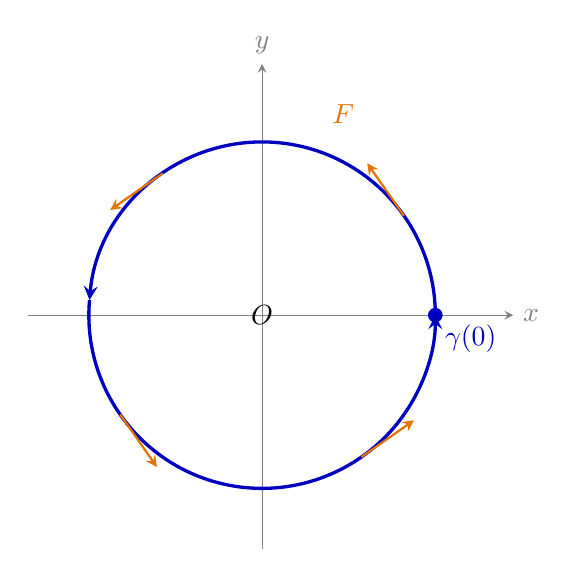
\begin{tikzpicture}[scale=2.2,>=stealth]
 \draw[->,gray] (-1.35,0)--(1.45,0) node[right] {$x$};
 \draw[->,gray] (0,-1.35)--(0,1.45) node[above] {$y$};
 \draw[blue!75!black,very thick,->] (0:1) arc (0:175:1);
 \draw[blue!75!black,very thick,->] (175:1) arc (175:360:1);
 \foreach \ang in {35,125,215,305}{
  \draw[orange!90!black,thick,->]
   ({cos(\ang)},{sin(\ang)})--
   ({cos(\ang)-.37*sin(\ang)},{sin(\ang)+.37*cos(\ang)});
 }
 \fill[blue!75!black] (1,0) circle (1.2pt);
 \node[blue!75!black,below right] at (1,0) {$\gamma(0)$};
 \node[orange!90!black,above right] at (0.35,1.05) {$F$};
 \node at (0,0) {$O$};
\end{tikzpicture}
\caption{Pole $F(x,y)=(-y,x)$ na okręgu jednostkowym
jest styczne i zgodne z dodatnią orientacją drogi.
Całka zmienia znak po odwróceniu orientacji
(przykład \ref{ma2:ex:line-circle-second}).}
\label{ma2:fig:line-circle}
\end{figure}

\begin{przyklad}[Pole o równych pochodnych mieszanych bez funkcji pierwotnej]
\label{ma2:ex:line-punctured-plane}
Na $U=\R^2\setminus\{(0,0)\}$ połóżmy
\[
 F(x,y)=\left(-\frac{y}{x^2+y^2},
 \frac{x}{x^2+y^2}\right).
\]
Pole jest gładkie na $U$ i
\[
 \partial_yF_1(x,y)=
 \frac{y^2-x^2}{(x^2+y^2)^2}
 =\partial_xF_2(x,y).
\]
Jednak dla $\gamma(t)=(\cos t,\sin t)$,
$0\le t\le2\pi$, mamy $F(\gamma(t))=\gamma'(t)$
oraz $W_\gamma(F)=2\pi$.
Z \ref{ma2:thm:line-path-independence}
wynika, że pole nie ma funkcji pierwotnej na $U$.
Hipotezy geometrycznej w
\ref{ma2:thm:line-star-shaped} nie można
zastąpić samą spójnością zbioru.
\end{przyklad}

\begin{przyklad}[Helisa i całka z pola zachowawczego]
\label{ma2:ex:line-helix}
Niech $\gamma(t)=(R\cos t,R\sin t,ht)$,
$0\le t\le T$, $R,T>0$, $h\in\R$.
Z \ref{ma2:ex:curve-helix} prędkość jest
stała i równa $\sqrt{R^2+h^2}$.
Dla $f(x,y,z)=x^2+y^2+z^2$ otrzymujemy
\[
 I_\gamma(f)=\sqrt{R^2+h^2}
 \left(R^2T+\frac{h^2T^3}{3}\right)
\]
przez całkowanie wielomianu w parametrze.
Jeżeli $F(x,y,z)=(x,y,z)$, to
$F=\nabla P$ dla $P(x,y,z)=(x^2+y^2+z^2)/2$.
Z \ref{ma2:thm:line-fundamental}
\[
 W_\gamma(F)=\frac{h^2T^2}{2}.
\]
Wynik można też otrzymać bezpośrednio:
$\langle F(\gamma(t)),\gamma'(t)\rangle=h^2t$.
\end{przyklad}

W dalszych rozdziałach zastosujemy całki
pierwszego rodzaju do obliczania wielkości
geometrycznych oraz rozszerzymy całkowanie
względem $\mathcal H^1$ na całki powierzchniowe
względem $\mathcal H^k$.
Twierdzenia Greena i Stokesa połączą
całki zorientowane po brzegach z całkami
po odpowiednich zbiorach.
